%auto-ignore
\documentclass[preview=false]{standalone}

\usepackage{graphics,graphicx,xcolor}
\usepackage{standalone}
\usepackage{tikz}
\usetikzlibrary{calc,shapes.arrows,decorations.pathreplacing,decorations.markings,arrows,positioning,patterns,shapes.multipart,automata, arrows.meta, positioning}

\definecolor{rouge}{RGB}{255,77,77}
\definecolor{vert}{RGB}{0,178,102}
\definecolor{jaune}{RGB}{255,255,0}
\definecolor{violet}{RGB}{208,32,144}
\definecolor{orange}{RGB}{255,140,0}
\definecolor{bleu}{RGB}{0,0,205}

%tuile de Wang: (x,y) et couleurs N,E,S,W
\newcommand{\wang}[6]{
\draw [black,fill=#3] (#1,#2+1)  -- (#1+0.5,#2+0.5) -- (#1+1,#2+1) -- cycle;
\draw [black,fill=#4] (#1+1,#2+1)  -- (#1+0.5,#2+0.5) -- (#1+1,#2) -- cycle;
\draw [black,fill=#5] (#1,#2)  -- (#1+0.5,#2+0.5) -- (#1+1,#2) -- cycle;
\draw [black,fill=#6] (#1,#2)  -- (#1+0.5,#2+0.5) -- (#1,#2+1) -- cycle;
}

\begin{document}

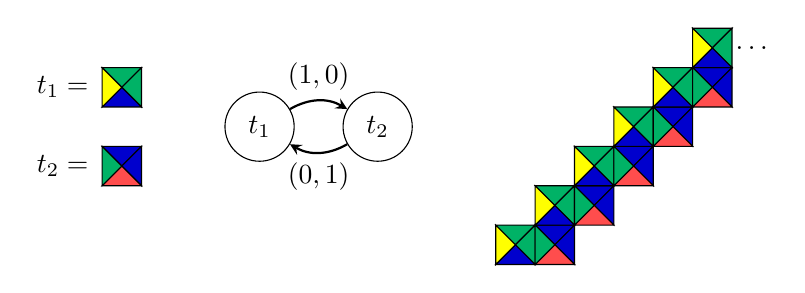
\begin{tikzpicture}[scale=0.5,node distance = 3cm, on grid, auto]

\begin{scope}[shift={(-4,0)}]
\draw (-1,0.5) node{$t_1=$};
\draw (-1,-1.5) node{$t_2=$};

\wang{0}{0}{vert}{vert}{bleu}{jaune} 
\wang{0}{-2}{bleu}{bleu}{rouge}{vert} 
\end{scope}

\node (t1) [state] at (0,-0.5) {$t_1$};
\node (t2) [state] at (3,-0.5) {$t_2$};

\path [-stealth, thick]
    (t1) edge [bend left] node {$(1,0)$} (t2)
    (t2) edge [bend left] node {$(0,1)$} (t1);

\begin{scope}[shift={(3,0)}]
% \draw[step=1cm,black,very thin] (2,-5) grid (10,3);
\wang{3}{-4}{vert}{vert}{bleu}{jaune} 
\wang{4}{-4}{bleu}{bleu}{rouge}{vert} 
\wang{4}{-3}{vert}{vert}{bleu}{jaune} 
\wang{5}{-3}{bleu}{bleu}{rouge}{vert} 
\wang{5}{-2}{vert}{vert}{bleu}{jaune} 
\wang{6}{-2}{bleu}{bleu}{rouge}{vert} 
\wang{6}{-1}{vert}{vert}{bleu}{jaune} 
\wang{7}{-1}{bleu}{bleu}{rouge}{vert}  
\wang{7}{0}{vert}{vert}{bleu}{jaune} 
\wang{8}{0}{bleu}{bleu}{rouge}{vert} 
\wang{8}{1}{vert}{vert}{bleu}{jaune} 
\draw (9.5,1.5) node{$\dots$};
\end{scope}


\end{tikzpicture}

\end{document}
